\documentclass[answers,addpoints]{exam}
\usepackage[margin=10mm]{geometry}
\usepackage{amsthm}
\usepackage{float} %  figure inside minipage 
\usepackage{ifthen,empheq}
\usepackage[]{graphicx}
\usepackage[]{minted}
\usepackage{amssymb}
\usepackage[multidot]{grffile}
\usepackage{pgfplots}
\usepackage{pgfplotstable}
\setlength{\headheight}{20pt}

\usepackage{tikz}
\usepgfplotslibrary{external}
\tikzexternalize[prefix=_tikz/,shell escape=-shell-escape]
\tikzset{external/system call={pdflatex \tikzexternalcheckshellescape -halt-on-error -interaction=batchmode -jobname "\image" "\texsource"}}
\immediate\write18{mkdir -p _tikz}

\title{Solution to HW2}
\author{Dilawar Singh}
\usepackage{hyperref}

\begin{document}
\Large
\maketitle

\begin{questions}

    \question{20 Marks}

    Refer to homework.

    \begin{solution}

        Except for the last subplot, these plots shows how each function
        will transform given functions in homework. These two functions are in
        first subplot. They are called \texttt{fun1} and \texttt{fun2}.

        \begin{figure}[H]
        \begin{center}
            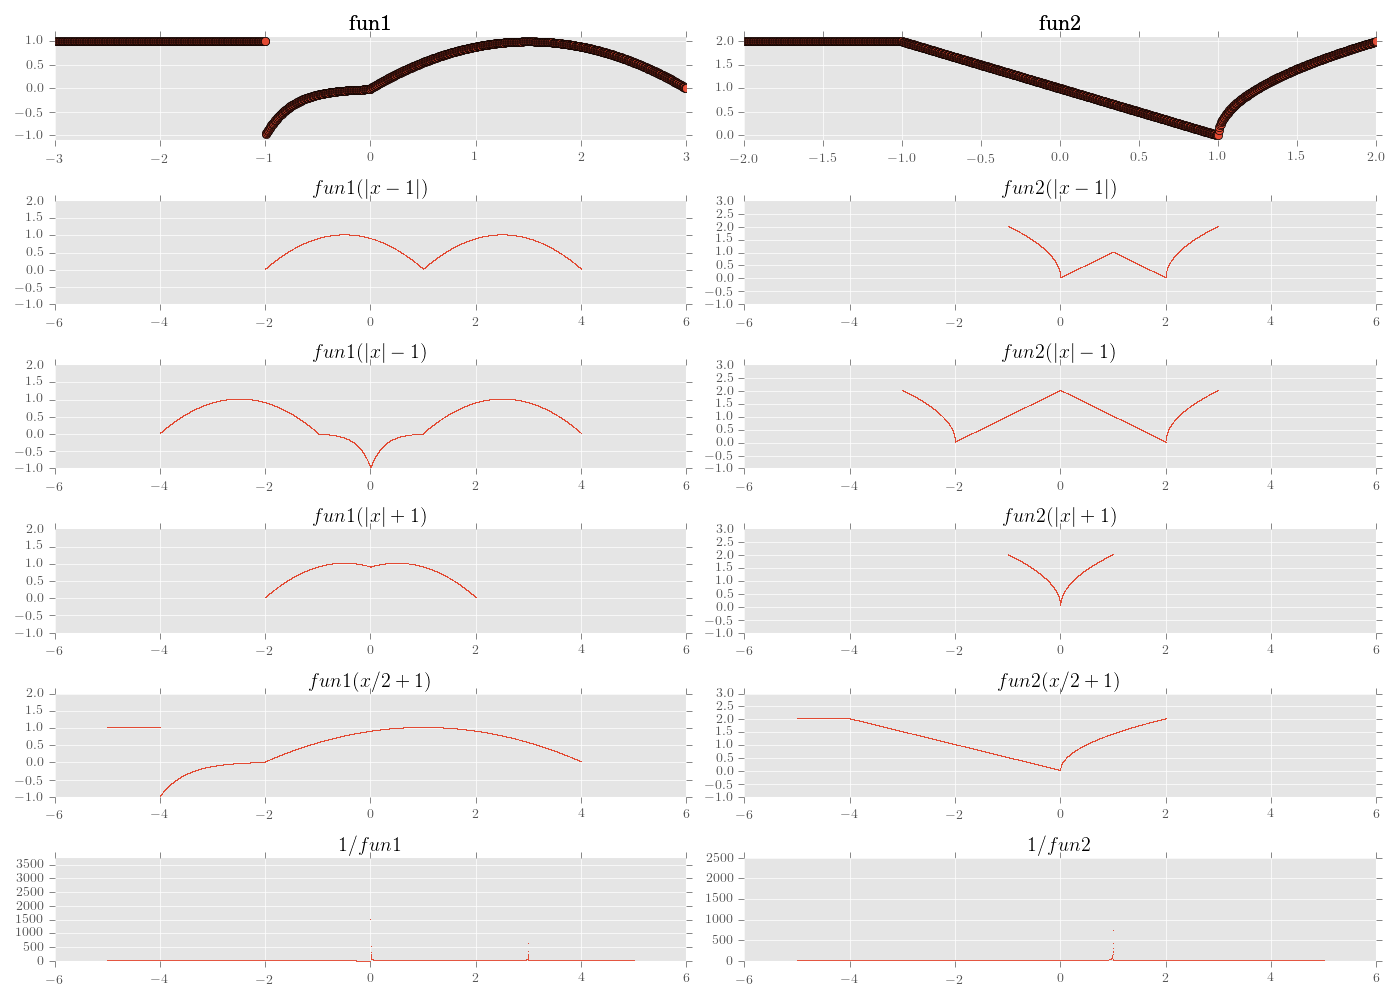
\includegraphics[width=1\textwidth]{./solution1.png}
        \end{center}
        \caption{Solution to problem 1}
        \label{fig:}
        \end{figure}

    \end{solution}

\end{questions}

\end{document}          
